\section{Grammatiche Attribute}
SDD (Syntax Directed Definition)
SDT (Syntax Directed Translation)

Aggiungo alla grammatica degli attributi e delle regole per quest'utlimi.
(Desc Calculator) posso computare valori associati ad espressioni aritmetiche.

%%%%%%%%%%%%%%%%%%%%%%%%%%%%%%%%%%%%%%%%%%%%%%%%%%%%%%%%%%%%%%%%%%%%%%%%%%%%
\subsection{Esempio}
\begin{tabular}{l}
	$E \rightarrow E + T | T$\\
	$T \rightarrow T * F | F$\\
	$F \rightarrow (E) | id$\\
\end{tabular}

Associo attributi ai terminali e non terminali, che recupero dall'analisi lessicale.

\begin{center}
	$3 + 4 * 5$ \\
	\Tree[. E [.E [.T [.F [.id (3) ] ] ] ] + [.T [.T [.F [.id (4) ] ] ] * [.F [.id (5) ] ] ] ]\\
\end{center}


Faccio visita postorder dell'albero (Bottom Up), associo i valori degli attributi a id, poi a F, poi risalgo a T. Quando sonon in T * F, T=4, F=5;
Quindi risolvo 4*5 che assegno come attributo al nodo padre T.

\begin{tcolorbox}\begin{center}
	\textbf{E.val} per indicare l'attributo della E.
\end{center}\end{tcolorbox}

\begin{tabular}{ll}
	$ \$\$ $ 	& Il driver\\
	$ \$ 1 $	& Primo elemento della produzione\\
\end{tabular}	 

$E_1 \rightarrow E_2 + T$ $\{ E_1.val = E_2.val + T.val \} $ \textbf{azione semantica} \\
$E \rightarrow T$ $\{ E.val = T.val \} $ \\
$T_1 \rightarrow T_2 * F $ $\{ T_1.val = T_2.val + F.val \} $ \\
$T \rightarrow F $ $ T.val = F.val $ \\
$F \rightarrow (E) $ $\{ F.val = E.val \} $ \\
$F \rightarrow id $ $\{ F.val = lexval(id) \} $ \\

Abstract Syntax Tree (albero derivazione \lq\lq ristretto\rq\rq )
\Tree[.+ $id_3$ [.* $id_4$ $id_5$ ] ]

\subsection{Attributi sintetizzati}
$A \rightarrow \alpha $ A.a definito come una funzione degli attributi dei terminali e non terminali in $\alpha $.
Gli attributi dei terminali derivano dall'analisi lessicale.

\subsection{Esempio, dichiarazione variabili}
\begin{lstlisting}
	int pippo, pluto, paperino;
\end{lstlisting}

$D \rightarrow TL$ $\{ L.i = T.t \} $\\
$T \rightarrow int$ $\{ T.t = integer\} $\\
$T \rightarrow float$ $\{ T.t = float \} $\\
$L_1 \rightarrow L_2,\ id$ $\{ L_2.i = L_1.i,\ addType(lex(id), L_1.i) \} $\\
$L \rightarrow id$ $\{ addType(lex(id)),\ L_i) \} $\\

\Tree[.D [.T int ] [.L [.L [.L [.id (pluto) ] ] , [.id (pippo) ] ] , [.id (paperino) ] ] ]

\begin{center}
	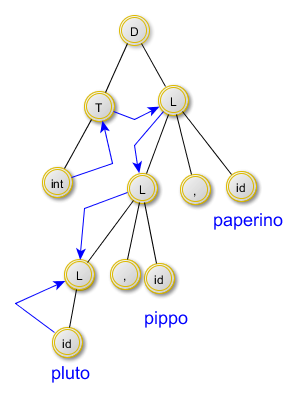
\includegraphics[scale=0.5]{Chapters/Img/l02_01.png}\\
\end{center} 

Gli attributi ereditati sono funzione degli attributi di siblings e del padre (driver della produzione).

\subsection{Example}
$S \rightarrow Number$\\
$Number \rightarrow o Digits$ serie di cifre in ottali (o)\\
$Number \rightarrow Digits d$\\
$Digits \rightarrow d$\\

\Tree[.N o [.Digits [.(...) d ] d ] ]

Gira l'albero!
$ S \rightarrow Digits $\\
$ Digits_1 \rightarrow Digits_2 d $ $\{ Digits_1.val = Digits_2 * Dg.tg_2.base + "d" \}$\\
$ Digits \rightarrow d $ $\{ Digit.base = 10; Digit.val = "d" \}$\\
$ Digits \rightarrow od $ $\{ Digit.base = 8; Digit.val = "d" \}$\\

Supponiamo per assurdo che sia LALR.